\chapter{Simple Template Language}
\label{Chapter: STL}

{\bf STL} is a template language. It is implemented as an XML namespace
handler, taking advantage of the underlying infrastructure provided by
{\tt itools.xml}.

{\bf STL} process and transforms XML files. It is aimed at presentation,
for example to produce the web pages that make up the user interface of
a web application.


\section{A descriptive language}

Unlike other template languages in the Python world, {\bf STL} does not
mix Python code within the template. The {\bf STL} statements only describe
the transformations to be performed on the template.

This way the logic and the presentation are really separated.

There are always two sides: the {\em template}, which represents the
presentation side; and the {\em namespace}, the logic side.

In five words: {\bf STL} is a {\em descriptive} language.

\subsection{The template}

For example, look at the template below ({\tt examples/chapter8/template.xml}):

\begin{code}
    <?xml version="1.0" encoding="UTF-8"?>
    <!DOCTYPE html
         PUBLIC "-//W3C//DTD XHTML 1.0 Transitional//EN"
         "http://www.w3.org/TR/xhtml1/DTD/xhtml1-transitional.dtd">
    <html xmlns="http://www.w3.org/1999/xhtml"
          xmlns:stl="http://xml.itools.org/namespaces/stl">
      <head></head>
      <body>
        <h1 stl:content="title" />
      </body>
    </html>
\end{code}

Note the declaration of the {\em stl} namespace, it is mandatory.

When this template will be processed, the content of the {\tt <h1>} tag
will be replaced by the value of the variable {\tt title}. But, where will
we find {\tt title}? Solution: in the namespace.

\subsection{The namespace}

In order to process an {\bf STL} template, you need to pass it a Python
namespace (a dictionary for example). But first we have to load the template
as a handler:

\begin{code}
    >>> from itools.handlers import get_handler
    >>> from itools import xml
    >>>   
    >>> template = get_handler('template.xml')
    >>> 
    >>> template
    <itools.xml.XML.Document object at 0x405ea38c>
\end{code}

Note that so far nothing delates the {\bf STL} presence, but inspecting
the {\tt template} object shows that the {\em stl} namespace handler has
been loaded:

\begin{code}
    >>> template.stl
    <itools.xml.STL.STL object at 0x406516cc>
\end{code}

Ok, it is time to build the namespace and process the template:

\begin{code}
    >>> namespace = {'title': 'hello world'}
    >>> print template.stl(namespace)
    <?xml version="1.0" encoding="UTF-8"?>
    <!DOCTYPE html
         PUBLIC "-//W3C//DTD XHTML 1.0 Transitional//EN"
        "http://www.w3.org/TR/xhtml1/DTD/xhtml1-transitional.dtd">
    <html xmlns:stl="http://xml.itools.org/namespaces/stl"
          xmlns="http://www.w3.org/1999/xhtml">
      <head></head>
      <body>
        <h1>hello world</h1>
      </body>
    </html>
\end{code}


As this example shows, the value of the variable {\tt title} is looked within
the namespace passed as parameter to {\tt template.stl}.


\section{Example: Task Tracker}

Now we are going to illustrate {\bf STL} with a more complex example.
Building up on the Task Tracker from the Chapter~\ref{section: files2},
we are going to write a method that produces an HTML page showing all
the tasks.

First, the template (see {\tt examples/chapter8/TaskTracker\_view.xml}):

\begin{code}
    <?xml version="1.0" encoding="UTF-8"?>
    <!DOCTYPE html
         PUBLIC "-//W3C//DTD XHTML 1.0 Transitional//EN"
         "http://www.w3.org/TR/xhtml1/DTD/xhtml1-transitional.dtd">
    <html xmlns="http://www.w3.org/1999/xhtml"
          xmlns:stl="http://xml.itools.org/namespaces/stl">
      <head></head>
      <body>
        <h2>Task Tracker</h2>
        <div stl:repeat="task tasks">
          <h4>
            #<stl:block content="task/id" />:
            <stl:block content="task/title" />
            (<em stl:content="task/state" />)
          </h4>
          <p stl:content="task/description" />
        </div>
      </body>
    </html>
\end{code}

The first new thing this example shows is the {\tt repeat} statement. While
{\tt stl:content} expects a string as the value, {\tt stl:repeat} expects a
sequence. When this template is processed, the XML output will contain as
many {\tt <div>} elements as tasks are in the {\tt tasks} variable. Within
the div element, in each iteration over the {\tt tasks} sequence, the
variable {\tt task} will be the respective item of the list.

The second new thing we see is the {\tt <stl:block>} element. When the
template is processed the {\tt <stl:block>} tags are automatically
removed.

Finally, look at the expression {\tt task/id} or {\tt task/title}, it shows
the {\em slash} operator, which lets to traverse namespaces. So the variable
{\tt task} is expected to be a mapping (e.g. a dictionary), and
{\tt id} a key in that mapping, whose value is a string.

\subsubsection{The Python side}

Now let's see the Python code (see {\tt examples/chapter8/TaskTracker.py}).
Basically we have added the method {\tt view} to the class {\tt TaskTracker}:

\begin{code}
    def view(self):
        # Load the STL template
        handler = get_handler('TaskTracker_view.xml')

        # Build the namespace
        namespace = {}
        namespace['tasks'] = []
        for i, task in enumerate(self.tasks):
            namespace['tasks'].append({'id': i,
                                       'title': task.title,
                                       'description': task.description,
                                       'state': task.state,
                                       'is_open': task.state == 'open'})

        # Process the template and return the output
        return handler.stl(namespace)
\end{code}

To try the code run the Python interpreter and type:

\begin{code}
    >>> from itools.handlers import get_handler
    >>> import TaskTracker
    >>> 
    >>> task_tracker = get_handler('itools.tt')
    >>> print task_tracker.view()
    <?xml version="1.0" encoding="UTF-8"?>
    <!DOCTYPE html
         PUBLIC "-//W3C//DTD XHTML 1.0 Transitional//EN"
        "http://www.w3.org/TR/xhtml1/DTD/xhtml1-transitional.dtd">
    <html xmlns:stl="http://xml.itools.org/namespaces/stl"
          xmlns="http://www.w3.org/1999/xhtml">
      <head></head>
      <body>
        <h2>Task Tracker</h2>
        <div>
          <h4>
            #0:
            Re-write the chapter about writing handler classes.
            (<em>closed</em>)
          </h4>
          <p>A new chapter...
\end{code}

The Figure~\ref{Figure: task tracker} shows how the HTML looks with a
browser.

\begin{figure}
  \center
  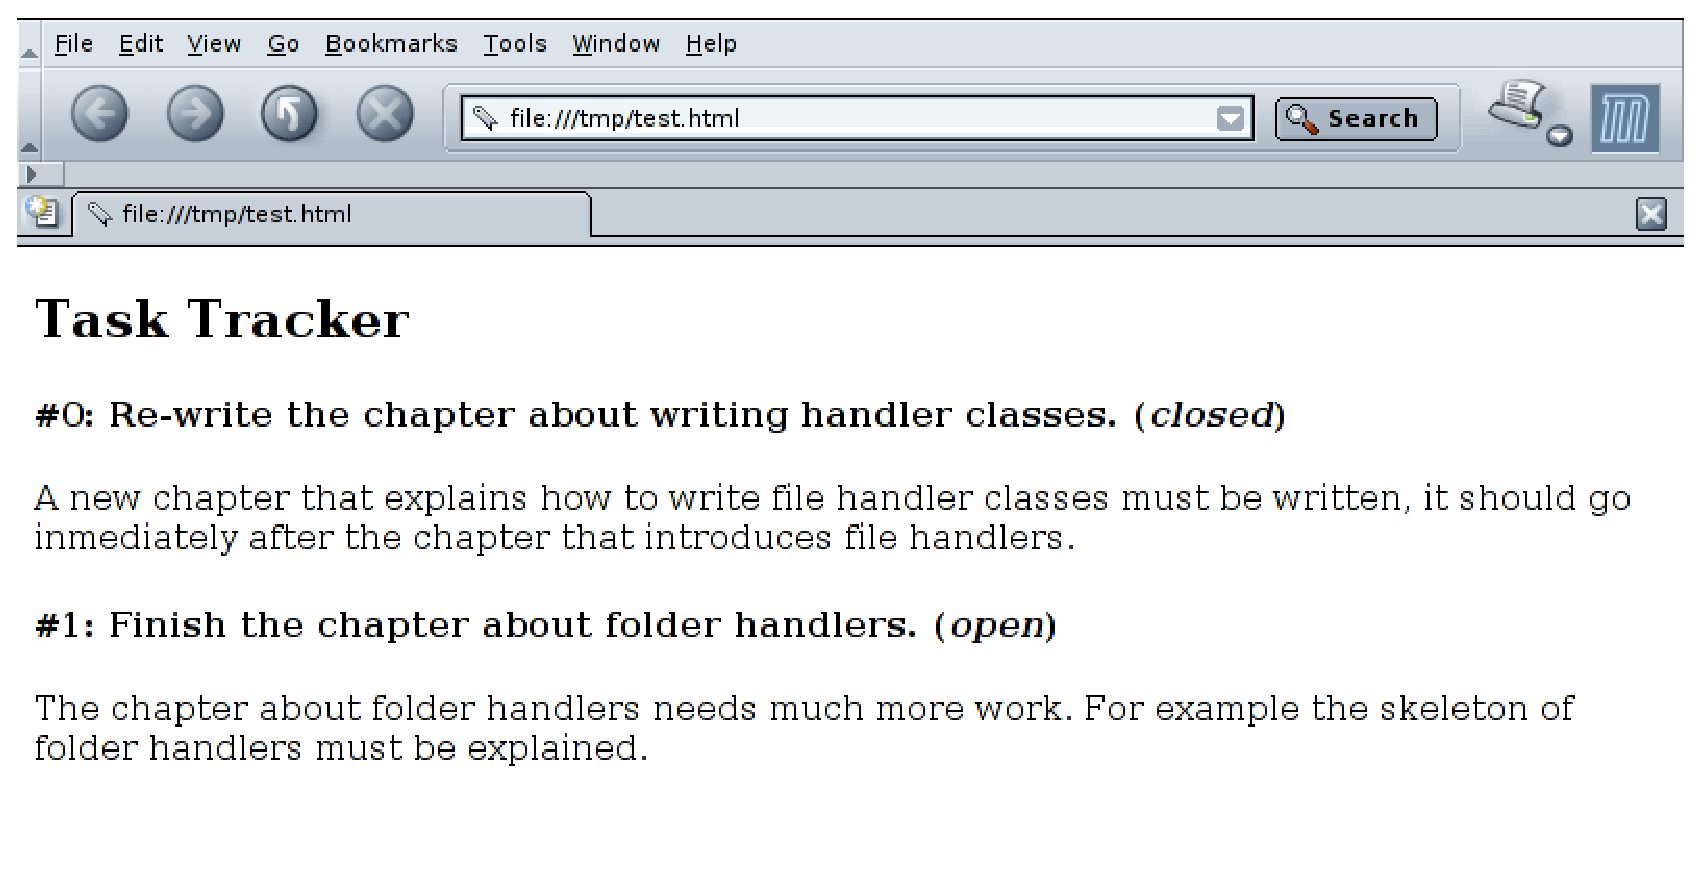
\includegraphics[width=\textwidth]{task_tracker.eps}
  \caption{The task tracker view}
  \label{Figure: task tracker}
\end{figure}



\section{Language overview}

So far we have seen {\tt stl:content} and {\tt stl:repeat}. Below is the
summary with all the {\bf STL} statements:

\begin{api}
    {\tt content}=``{\em expression}''\\
    - Replaces the element's content by the result of evaluating the given
    {\bf STL} expression.

    {\tt attributes}=``{\em name expression}[; {\em name expression}]*''\\
    - For every pair ``{\em name: expression}'', replace the the value of
    the attribute {\em name} by the result of evaluating {\em expression}.

    {\tt if}=``[not ]{\em expression}''\\
    - If the given expression evaluates to {\tt True}, do nothing; if
    evaluates to {\tt False}, remove the XML element.

    {\tt repeat}=``{\em name expression}''\\
    - The given expression is expected to be a sequence or an iterator.
    For every item in {\em expression}, create an element and add the
    item to the namespace stack before processing the element.
\end{api}


\subsection{Expressions}

The {\bf STL} expressions are pretty simple, their syntax is:

\begin{quote}
    name[/name]*
\end{quote}

That is, a sequence of names separated by slashes. The semantics is:

\begin{enumerate}
  \item Look the first name in the namespace stack.

  \item If there are more names left, the last value found must be a namespace,
    then look the next name in that namespace.

    Iterate until the last name is consumed.

  \item Once the end of the sequence is reached, we will have a value. If
    the value is callable, then call it to get a new value.

  \item Finally, we should have a value that is either a string, a boolean
    or a sequence, depending on which statement ({\tt content}, {\tt repeat},
    etc.) the expression is being used with.
\end{enumerate}



